\renewcommand{\FileName}{discrete}
\begin{comment}
\begin{frame}
  \frametitle{Discrete distributions}  
  \begin{itemize}
	\item {\large\bfseries Counts of occurrences:} accidents, words in text, 
	blood cells with some characteristic.
	\item{\large\bfseries Data:} Basic outcome value, \(k \,  , \,  k = 0 , 1, \dots\),
	and number of observations, \(n_k\), with that value.
	\item {\large\bfseries Example:} \emph{Federalist Papers}--- disputed authorship 
      \begin{itemize*}
	  \item 77 essays by Hamilton, Jay \& Madison: persuade NY voters to ratify Constitution, all
	  signed with pseudonym (``Publius'')
	  \item 65 known, 12 disputed (H \& M both claimed sole authorship)
	  \item \citet{MostellerWallace:84}: Analysis of frequency distributions of key ``marker'' words:
\emph{from}, \emph{may}, \emph{whilst}, $\dots$.
	  \item For each word, fit probability model (Poisson, NegBin)
$\rightarrow (\beta_1, \beta_2, \cdots) \longrightarrow $
log Odds (Hamilton vs. Madison)
	  \end{itemize*}
  \end{itemize}

  %\begin{table}[htb]
% \caption{Number of occurrences ($k$) and number of blocks of text ($n_k$) of the word \emph{may} in 
%essays written by  Madison}\label{tab:madison}
 \begin{center}
 \begin{tabular}{l|rrrrrrr}
  \hline
  Occurrences ($k$)   &   0 &  1 &  2 & 3 & 4 & 5 & 6 \\ 
      Blocks ($n_k$)  & 156 & 63 & 29 & 8 & 4 & 1 & 1 \\ 
  \hline
 \end{tabular}
 \end{center}
%\end{table}

\end{frame}
\end{comment}

\begin{frame}
  \frametitle{Discrete distributions}  
  \begin{itemize}
	\item {\large\bfseries Counts of occurrences:} accidents, words in text, 
	blood cells with some characteristic.
	\item{\large\bfseries Data:} Basic outcome value, \(k \,  , \,  k = 0 , 1, \dots\),
	and number of observations, \(n_k\), with that value.
	\item {\large\bfseries Example:} distributions of key ``marker''
	words: \emph{from}, \emph{may}, \emph{whilst}, $\dots$ in \emph{Federalist Papers}
	by James Madison, e.g., blocks of 200 words with  \emph{may}:

  %\begin{table}[htb]
% \caption{Number of occurrences ($k$) and number of blocks of text ($n_k$) of the word \emph{may} in 
%essays written by  Madison}\label{tab:madison}
 \begin{center}
 \begin{tabular}{l|rrrrrrr}
  \hline
  Occurrences ($k$)   &   0 &  1 &  2 & 3 & 4 & 5 & 6 \\ 
      Blocks ($n_k$)  & 156 & 63 & 29 & 8 & 4 & 1 & 1 \\ 
  \hline
 \end{tabular}
 \end{center}
%\end{table}


	\item {\large\bfseries Example:} Saxony
	families with 12 children having $k=0, 1, \dots 12$ sons.
  \end{itemize}
	
%\scalebox{.9}{%
%Unequal number of columns: 14 13
%\begin{table}[htb]
% \caption{Number of males in N=6115 Saxony families with 12 children}\label{tab:saxony}
 \begin{center}
 \setlength{\tabcolsep}{3pt}
 \begin{tabular}{l|rrrrrrrrrrrrr}
  \hline
  $k$ & 0 & 1 & 2 & 3 & 4 & 5 & 6 & 7 & 8 & 9 & 10 & 11 & 12 \\ 
  \hline
  $n_k$ & 3 & 24 & 104 & 286 & 670 & 1033 & 1343 & 1112 & 829 & 478 & 181 & 45 & 7 \\ 
  \hline
 \end{tabular}
 \end{center}
%\end{table}

%}
\end{frame}

\begin{frame}
  \frametitle{Discrete distributions}  

  \begin{block}{\large\bfseries Questions:}<1->
  	 \begin{itemize*}
  	 \item What process gave rise to the distribution?
  	 \item Form of distribution: uniform, binomial,
  	  Poisson, negative binomial, geometric, etc.?
  	 \item Estimate parameters
  	 \item Visualize goodness of fit
  	 \end{itemize*}
   \end{block}
  \begin{exampleblock}{\large\bfseries For example:}<2->
  	 \begin{itemize*}
  	 \item \emph{Federalist Papers:}  might expect a Poisson($\lambda$) distribution.
  	 \item \emph{Families in Saxony:}  might expect a Bin($n, p$) distribution 
  	 with $n=12$. Perhaps $p=0.5$ as well.
  	 \end{itemize*}
   \end{exampleblock}

\end{frame}

\begin{frame}
  \frametitle{Discrete distributions}  

  \begin{block}{\large\bfseries Lack of fit:}
	 \begin{itemize*}
     \item Lack of fit tells us something about the process giving rise to the data
     \item Poisson:  assumes constant small probability of the basic event
     \item Binomial: assumes constant probability and independent trials   
	 \end{itemize*}
  \end{block}

  \begin{exampleblock}{\large\bfseries Motivation:}
	 \begin{itemize*}
	   \item Models for more complex categorical data often use these basic discrete distributions
	   \item Binomial (with predictors) $\rightarrow$ logistic regression
	   \item Poisson (with predictors) $\rightarrow$ poisson regression, \loglin\ models 
	   \item $\Rightarrow$ many of these are special cases of \emph{generalized linear models}
	 \end{itemize*}

   \end{exampleblock}

\end{frame}

\subsection{Using SAS}
\begin{frame}
  \frametitle{Fitting and graphing discrete distributions}
  \begin{block}
      \VCD\ methods to fit, visualize, and diagnose discrete distributions:
  \end{block}

  \begin{itemize}
	\item{\large\bfseries Fitting:} \macro{GOODFIT} fits uniform, binomial,
 Poisson, negative binomial, geometric,  logarithmic series
 distributions (or any specified multinomial)

	\item{\large\bfseries Hanging rootograms:} Sensitively assess departure between Observed, Fitted
counts (\macro{ROOTGRAM})
	\item{\large\bfseries Ord plots:} Diagnose form of a discrete distribution (\macro{ORDPLOT})
	\item{\large\bfseries Poissonness plots:} Robust fitting and diagnostic plots for Poisson
(\macro{POISPLOT})
	\item{\large\bfseries Robust distribution plots} (\macro{DISTPLOT})
  \end{itemize}
\end{frame}

\subsection{Using SAS macros}
\begin{frame}[fragile]
  \frametitle{Sidebar: Using SAS macros}
  \begin{itemize}
    \item SAS macros are high-level, general programs consisting of a series of
	\texttt{DATA} steps and \texttt{PROC} steps.
	\item Keyword arguments substitute your data names, variable names, and
	options for the named macro parameters.
	\item Use as:
\begin{Code}
  %macname(data=dataset, var=variables, ...);
\end{Code}
	\item Most arguments have default values (e.g., \texttt{data=\_last\_})
	\item All \VCD\ macros have internal and online documentation,
	\url{http://datavis.ca/sasmac/}
	\item Macros can be installed in directories automatically searched by SAS.
	Put the following \texttt{options} statement in your \texttt{AUTOEXEC.SAS} file:
\begin{verbatim}
  options sasautos=('c:\sasuser\macros' sasautos);
\end{verbatim}

  \end{itemize}
\end{frame}

\begin{frame}[fragile]
  \frametitle{Sidebar: Using SAS macros}

E.g., the \macro{GOODFIT} is defined with the following arguments:
\vspace{1.5ex}
\begin{Input}[fontsize=\footnotesize,label=\fbox{$\cdots$ \texttt{goodfit.sas} $\cdots$},baselinestretch=0.8]
%macro goodfit(
  data=_last_,    \sascomment{/* name of the input data set             */}
  var=,           \sascomment{/* analysis variable (basic count)        */}
  freq=,          \sascomment{/* frequency variable                     */}
  dist=,          \sascomment{/* name of distribution to be fit         */}
  parm=,          \sascomment{/* required distribution parameters?      */}
  sumat=100000,   \sascomment{/* sum probs. and fitted values here      */}
  format=,        \sascomment{/* format for ungrouped analysis variable */}
  out=fit,        \sascomment{/* output fit data set                    */}
  outstat=stats); \sascomment{/* output statistics data set             */}
\end{Input}
Typical use:
\begin{Input}
%goodfit(data=madison, \sascomment{/* data set       */} 
    var=count,         \sascomment{/* count variable */}
    freq=blocks, 
    dist=poisson);
\end{Input}

\end{frame}

\subsection{Fitting discrete distributions} 
\begin{frame}
\frametitle{Fitting discrete distributions}
  \begin{itemize}
   \item {\large\bfseries Distributions:}
	 \begin{itemize*}
	   \item Poisson, $p(k) = e^{-\lambda }\lambda ^k/k!$
	   \item Binomial, $p(k) = \binom{n}{k} p^k(1-p)^{n-k}$
	   \item Negative binomial, $p(k) = \binom{n+k-1}{k}p^n(1-p)^k$
	   \item Geometric, $p(k) = p(1-p)^k$
	   \item Logarithmic series,  $p(k) = \theta ^k/[-k\log (1-\theta )]$
	 \end{itemize*}
  \item {\large\bfseries Estimate parameter(s):}
	 \begin{itemize*}
	   \item Poisson, $\hat\lambda = \sum k n_k / \sum n_k$ = mean
	   \item Binomial, $\hat p = \sum k n_k / (n \sum n_k)$ = mean / n
	 \end{itemize*}
  \item {\large\bfseries Goodness of fit:}
  \[
  \chi^2 = \sum_{k=1}^K \:
  \frac{{ ( n_k - N \hat{p}_k ) }^2}
  { N \hat{p}_k }  \sim \chi^2_{( K-1 )}
  \]
where \(\hat{p}_k\) is the estimated probability of each basic count,
under the hypothesis that the data follows the chosen distribution.
  \end{itemize}
\end{frame}

\begin{frame}[fragile]

\frametitle{\macrot{GOODFIT}: Fitting discrete distributions}
  \begin{itemize}
  \item \macro{GOODFIT} fits uniform, binomial,
   Poisson, negative binomial, geometric,  logarithmic series
   distributions (or any specified multinomial)
  \item E.g., Try fitting Poisson model
\end{itemize}

\vspace{1.5ex}
\begin{Input}[fontsize=\small,label=\fbox{\texttt{madfit.sas}},baselinestretch=0.8]
title "Instances of 'may' in Federalist papers";
data madison;
   input count blocks;
   label count='Number of Occurrences'
         blocks='Blocks of Text';
datalines;
  0    156
  1     63
  2     29
  3      8
  4      4
  5      1
  6      1
;
 %goodfit(data=madison, var=count, freq=blocks,  
      \sasemph{dist=poisson});
\end{Input}

\end{frame}

\begin{frame}[fragile]
\frametitle{Fitting discrete distributions}
The \macro{GOODFIT} gives a table of observed and fitted frequencies,
Pearson $\chi^2$ residuals (\texttt{CHI}) and likelihood-ratio deviance 
residuals (\texttt{DEV}).

\begin{Output}[gobble=2,fontsize=\footnotesize]
              Instances of 'may' in Federalist papers
 
   COUNT    BLOCKS      PHAT         EXP       CHI         DEV
 
     0        156     0.51867    135.891     1.72499     6.56171
     1         63     0.34050     89.211    -2.77509    -6.62056
     2         29     0.11177     29.283    -0.05231    -0.75056
     3          8     0.02446      6.408     0.62890     1.88423
     4          4     0.00401      1.052     2.87493     3.26912
     5          1     0.00053      0.138     2.31948     1.98992
     6          1     0.00006      0.015     8.01267     2.89568
            ======    =======    =======
              262     0.99999    261.998
\end{Output}
\end{frame}

\begin{frame}[fragile]
\frametitle{Fitting discrete distributions}
In addition, it provides the overall goodness-of-fit tests:
\begin{Output}[gobble=7]
         Goodness-of-fit test for data set MADISON
 
         Analysis variable:       COUNT Number of Occurrences
         Distribution:            POISSON
         Estimated Parameters:    lambda = 0.6565
 
         Pearson chi-square    = 88.92304707
         Prob > chi-square     = 0
 
         Likelihood ratio G2   = 25.243121314
         Prob > chi-square     = \sasemph{0.0001250511}
 
         Degrees of freedom    = 5
\end{Output}
The poisson model does not fit!  Why?
\end{frame}

\begin{frame}[fragile]

  \frametitle{What's wrong with histograms?}
  \begin{itemize}
  \item Discrete distributions often graphed as histograms, with a 
  theoretical fitted distribution superimposed.
%  \item E.g., Try fitting Poisson model

  \begin{Code}
   %goodfit(data=madison, var=count, freq=blocks,  
      \sasemph{dist=poisson});
  \end{Code}

  \end{itemize}

 \begin{minipage}[c]{.49\dispwidth}
  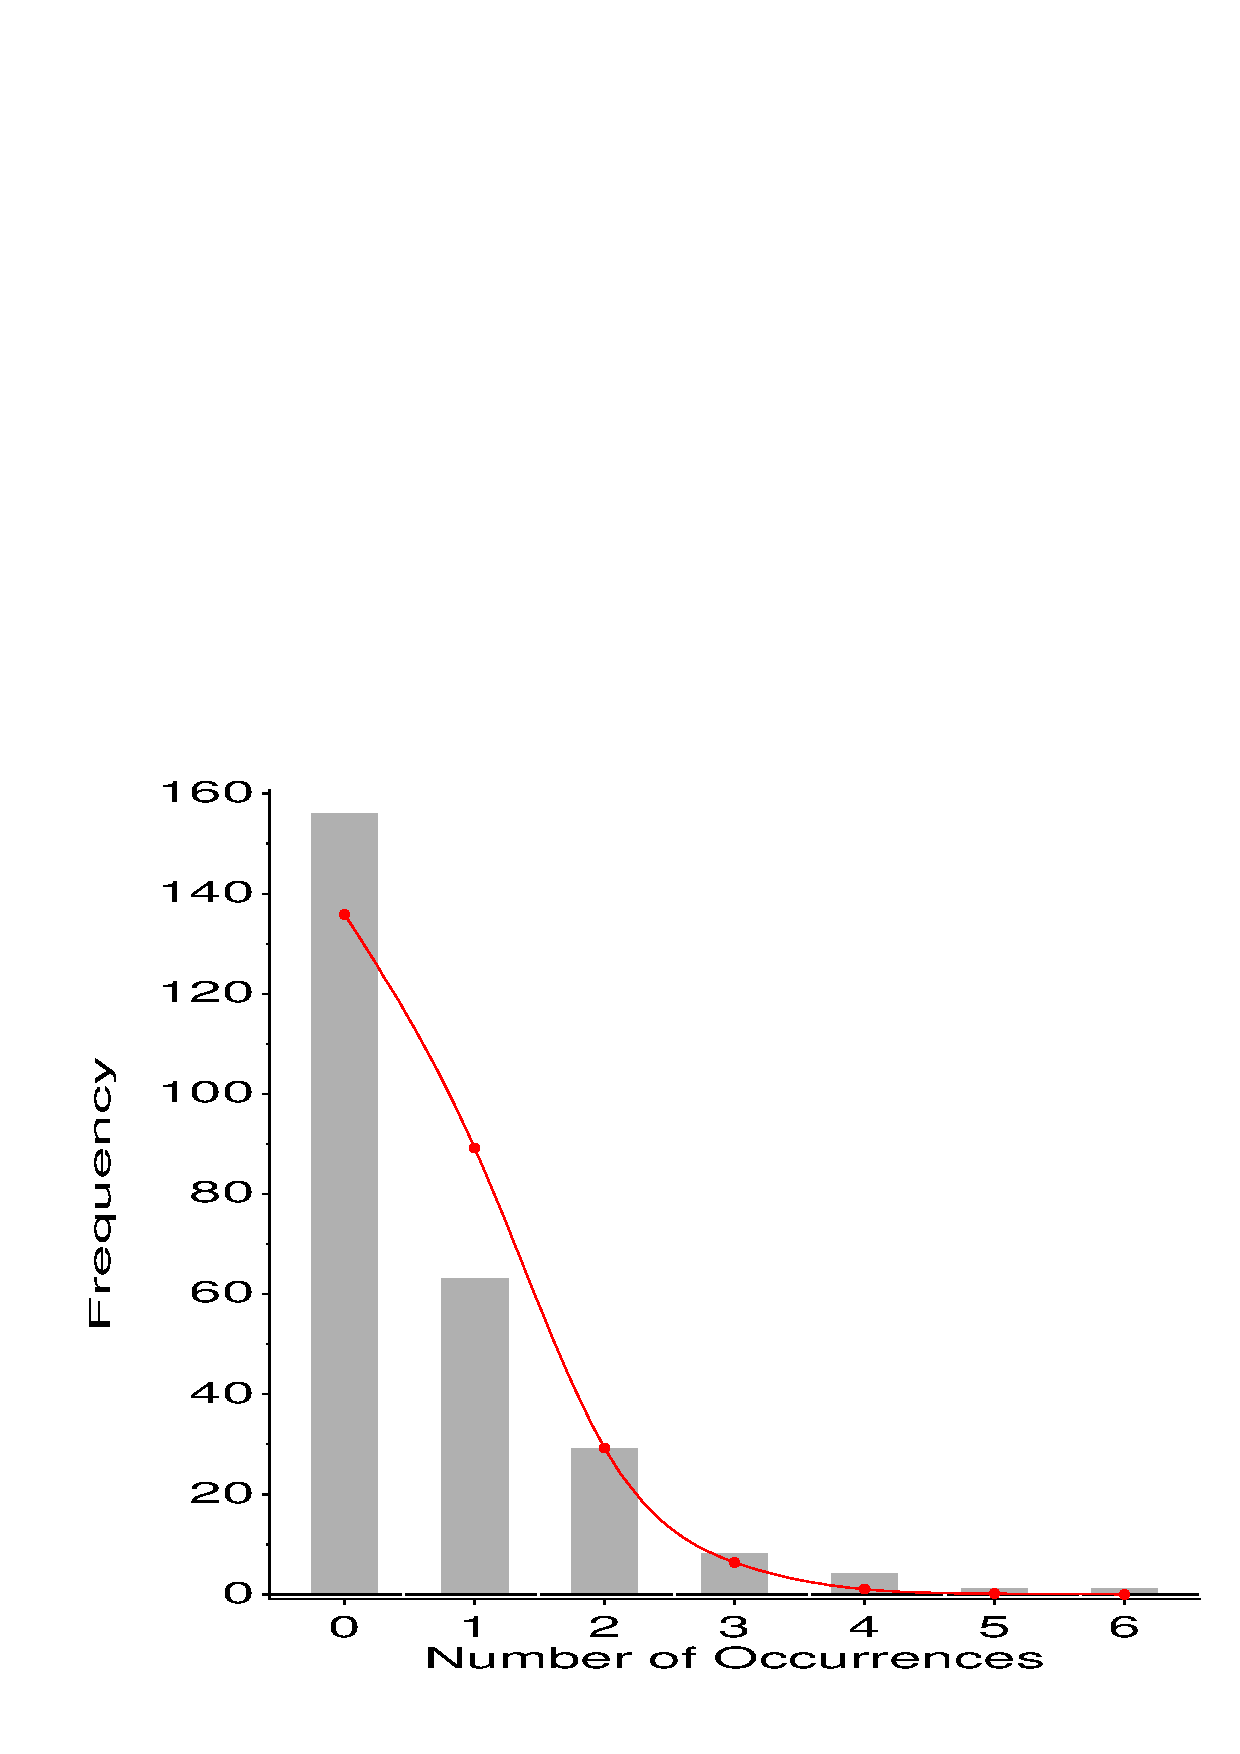
\includegraphics[width=1\linewidth]{fig/madfit1}
 \end{minipage}%
 \hfill
 \begin{minipage}[c]{.49\dispwidth}
 Problems:
	\begin{itemize*}
	\item largest frequencies dominate display
	\item must assess deviations vs. a curve
	\end{itemize*}
 \end{minipage}
	
\end{frame}

\begin{frame}[fragile]
  \frametitle{Hang \& root them $\rightarrow$ Hanging rootograms}
  \citet{Tukey:72,Tukey:77}:
  \begin{itemize*}
  \item shift histogram bars to 
  the fitted curve $\rightarrow$ judge deviations vs. horizontal line.
  \item plot $\sqrt{\mbox{freq}} \rightarrow$
  smaller frequencies are emphasized.
  \end{itemize*}

  \begin{Code}
   %goodfit(data=madison, var=count, freq=blocks, 
     dist=poisson, \sasemph{out=fit});
   \sasemph{%rootgram(data=fit, var=count, obs=blocks);}
  \end{Code}
    \begin{center}
	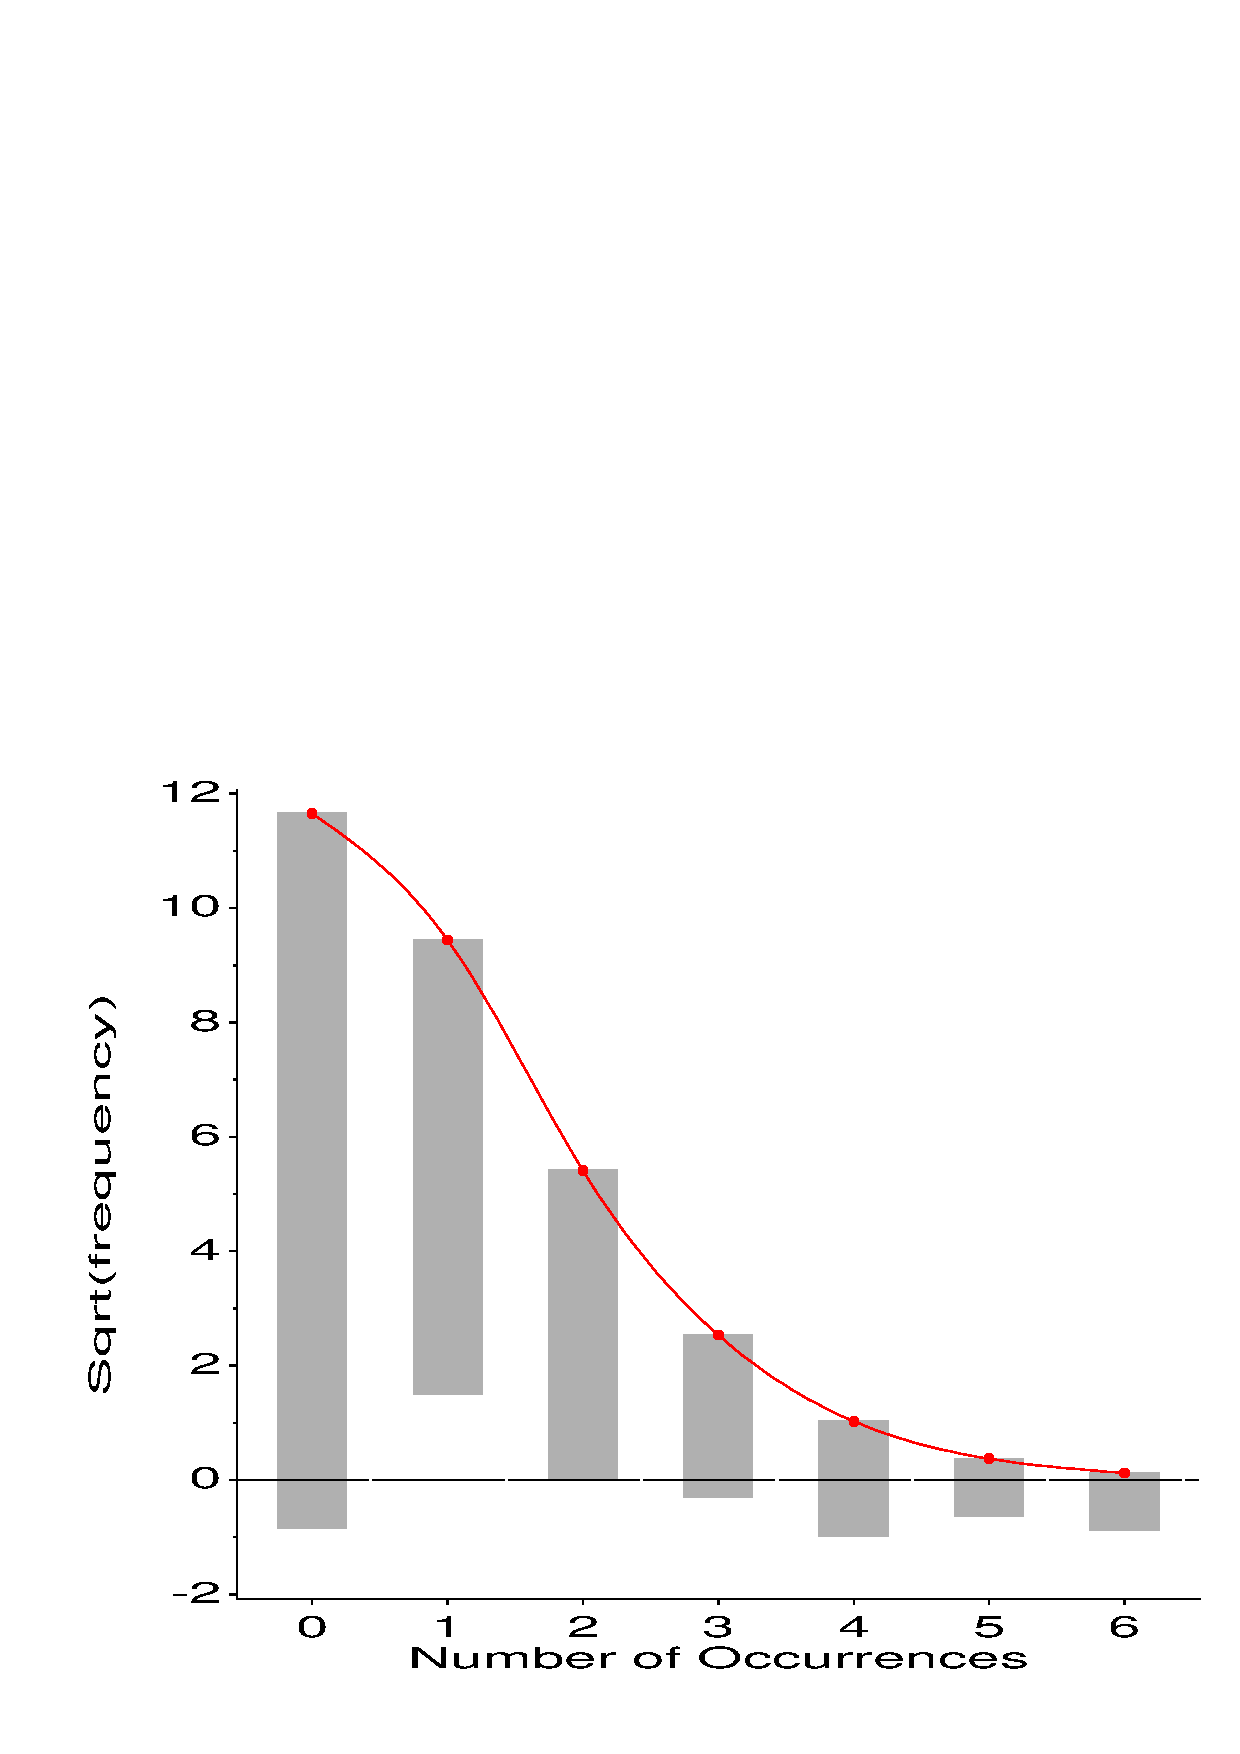
\includegraphics[width=.45\dispwidth,clip]{fig/madfit3}
    \end{center}

\end{frame}

\begin{frame}[fragile]
  \frametitle{Highlight differences $\rightarrow$ Deviation rootograms}
  \begin{itemize*}
  \item Emphasize differences between observed and fitted frequencies
  \item Draw bars to show the gaps (\texttt{btype=dev})
  \end{itemize*}

  \begin{Code}
   %goodfit(data=madison, var=count, freq=blocks, 
     dist=poisson, out=fit);
   %rootgram(data=fit, var=count, obs=blocks, \sasemph{btype=dev});
  \end{Code}
    \begin{center}
	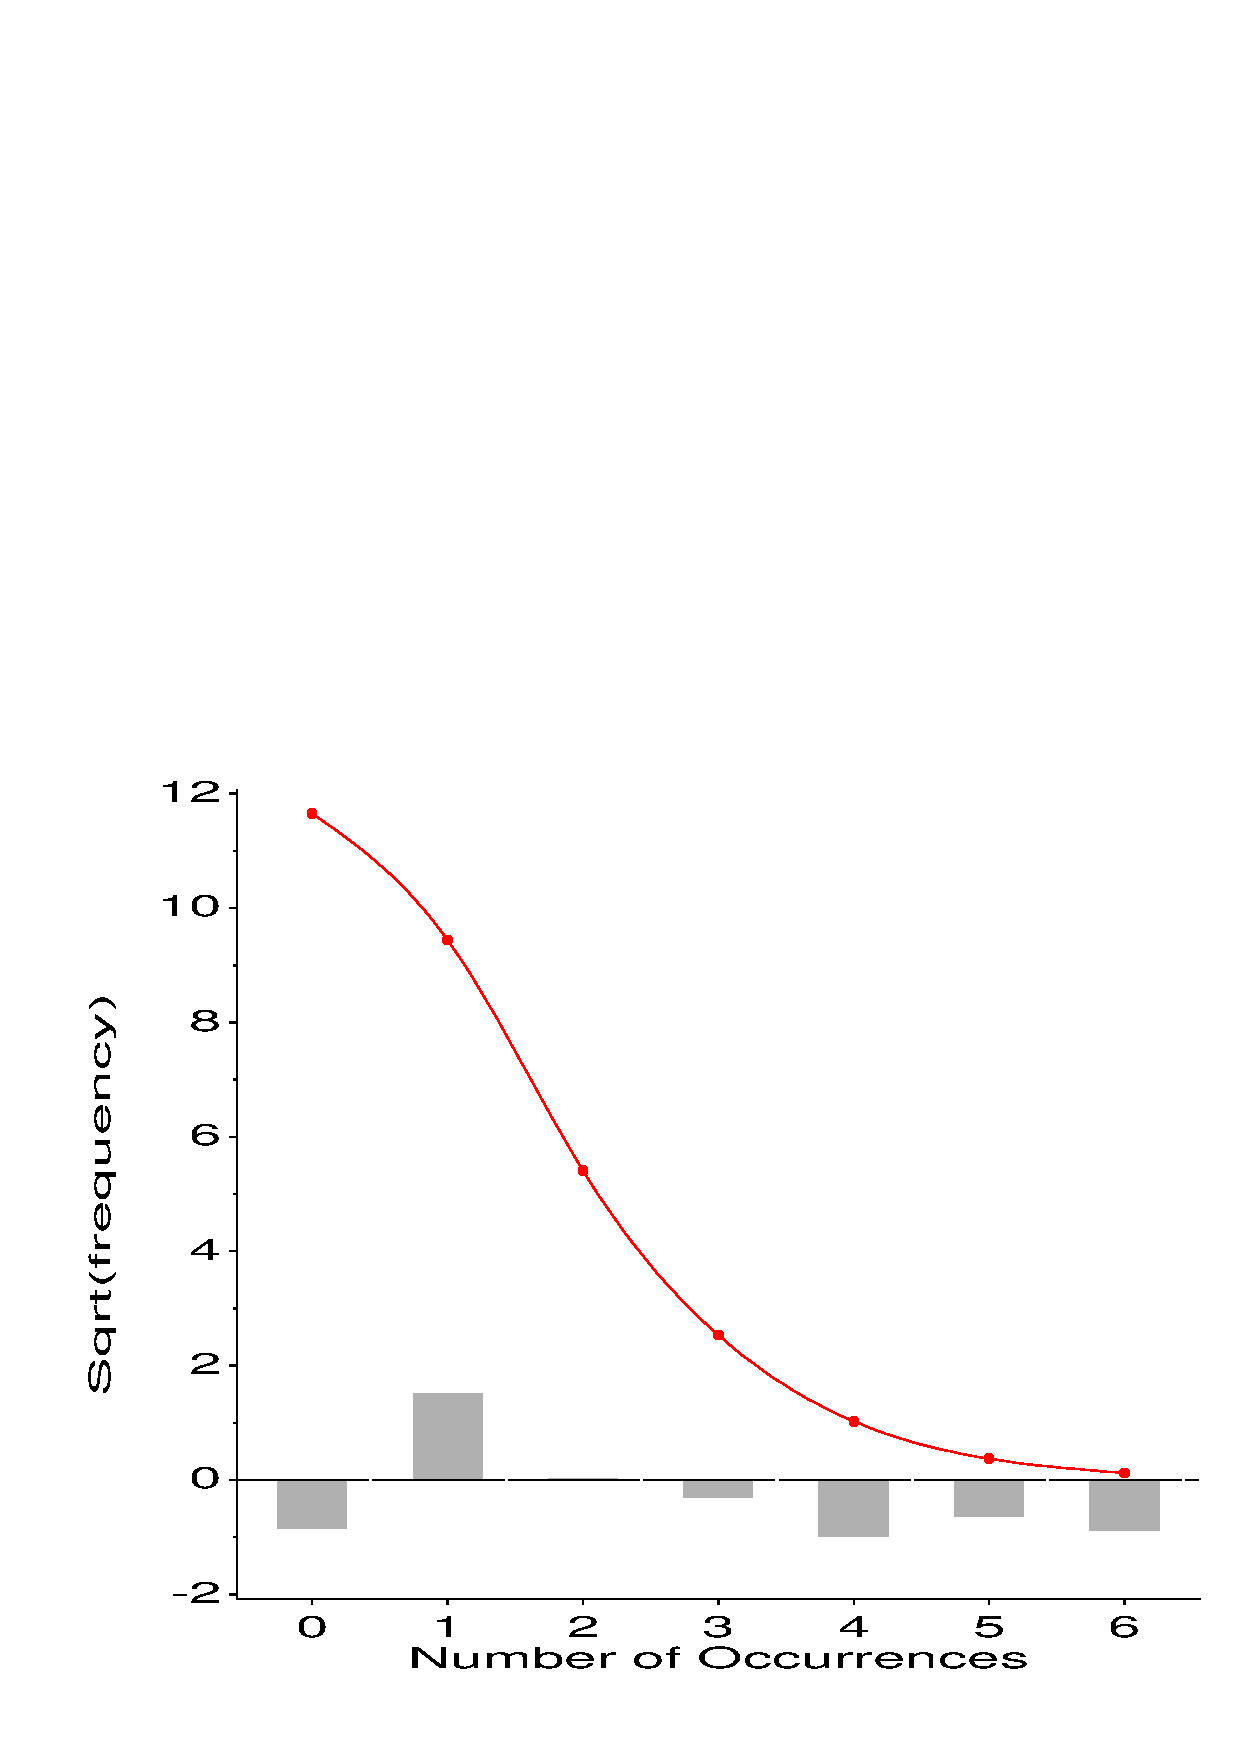
\includegraphics[width=.45\dispwidth,clip]{fig/madfit4}
    \end{center}

\end{frame}

\subsection{Ord plots: diagnose form}
\begin{frame}

\frametitle{Ord plots: Diagnose form of discrete distribution}
\begin{itemize}
\item How to tell which discrete distributions are likely candidates?
\item \citet{Ord:67}: for each of Poisson, Binomial, Negative Binomial, and Logarithmic Series distributions,
	\begin{itemize*}
	\item plot of $k p_k / p_{k-1}$ against $k$ is linear
	\item signs of intercept and slope $\rightarrow$ determine the form,
	give rough estimates of parameters
	\end{itemize*}

\begin{center}
%\vspace{1ex}
\renewcommand{\arraystretch}{.85}
\begin{tabular}{|ccll|}\hline
Slope & Intercept & Distribution & Parameter \\
(b)   & (a)       & (parameter)  &  estimate \\ \hline
0     &  $+$      &  Poisson (\(\lambda\)) & \(\lambda = a\)    \\
$-$   &  $+$      &  Binomial (n, p)       & \(p = b / (b-1)\)  \\
$+$   &  $+$      &  Neg. binomial (n,p)      & \(p = 1 - b\)      \\
$+$   &  $-$      &  Log.\ series (\(\theta\)) & \(\theta =  b\) \\
      &      &                     &   \(\theta = - a\) \\ \hline
\end{tabular}
\end{center}

\item Fit line by WLS, using $\sqrt{n_k-1}$ as weights
\end{itemize}
\end{frame}

\begin{frame}[fragile]
\frametitle{Ord plots}
\begin{itemize}
\item \macro{ORDPLOT}
\begin{Code}
 %ordplot(data=madison, count=Count, freq=blocks);
\end{Code}
\end{itemize}

 \begin{minipage}[c]{.4\dispwidth}
	\begin{itemize*}
	\item Diagnoses distribution as NegBin
	\item Estimates $\hat{p} = 0.576$
	\end{itemize*}
 \end{minipage}
 \hfill
 \begin{minipage}[c]{.59\dispwidth}
  \begin{center}
  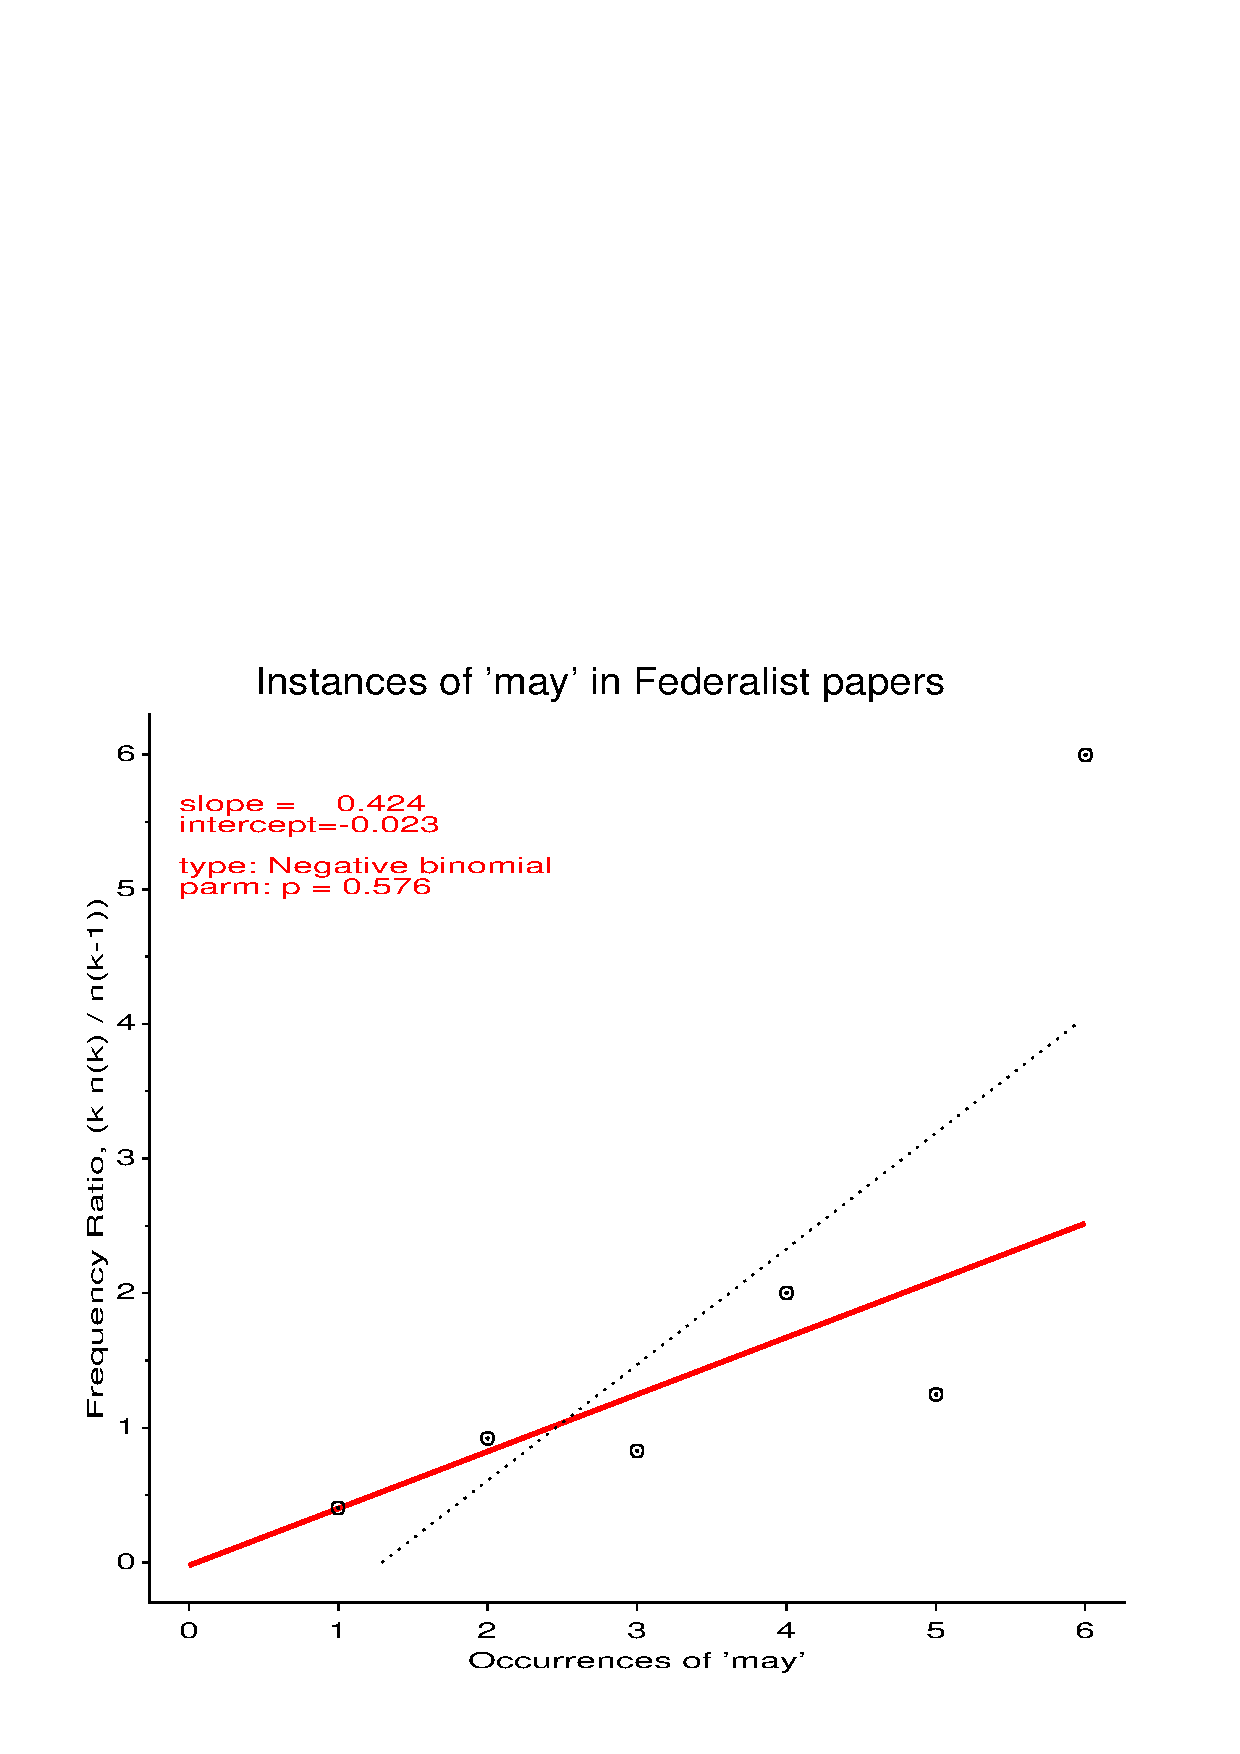
\includegraphics[trim=0 0 0 30,width=\linewidth,clip]{fig/orddemo2}
  \end{center}
 \end{minipage}
\end{frame}
	

\begin{frame}
\frametitle{Ord plots: Other distributions}

 \begin{minipage}[c]{.49\dispwidth}
  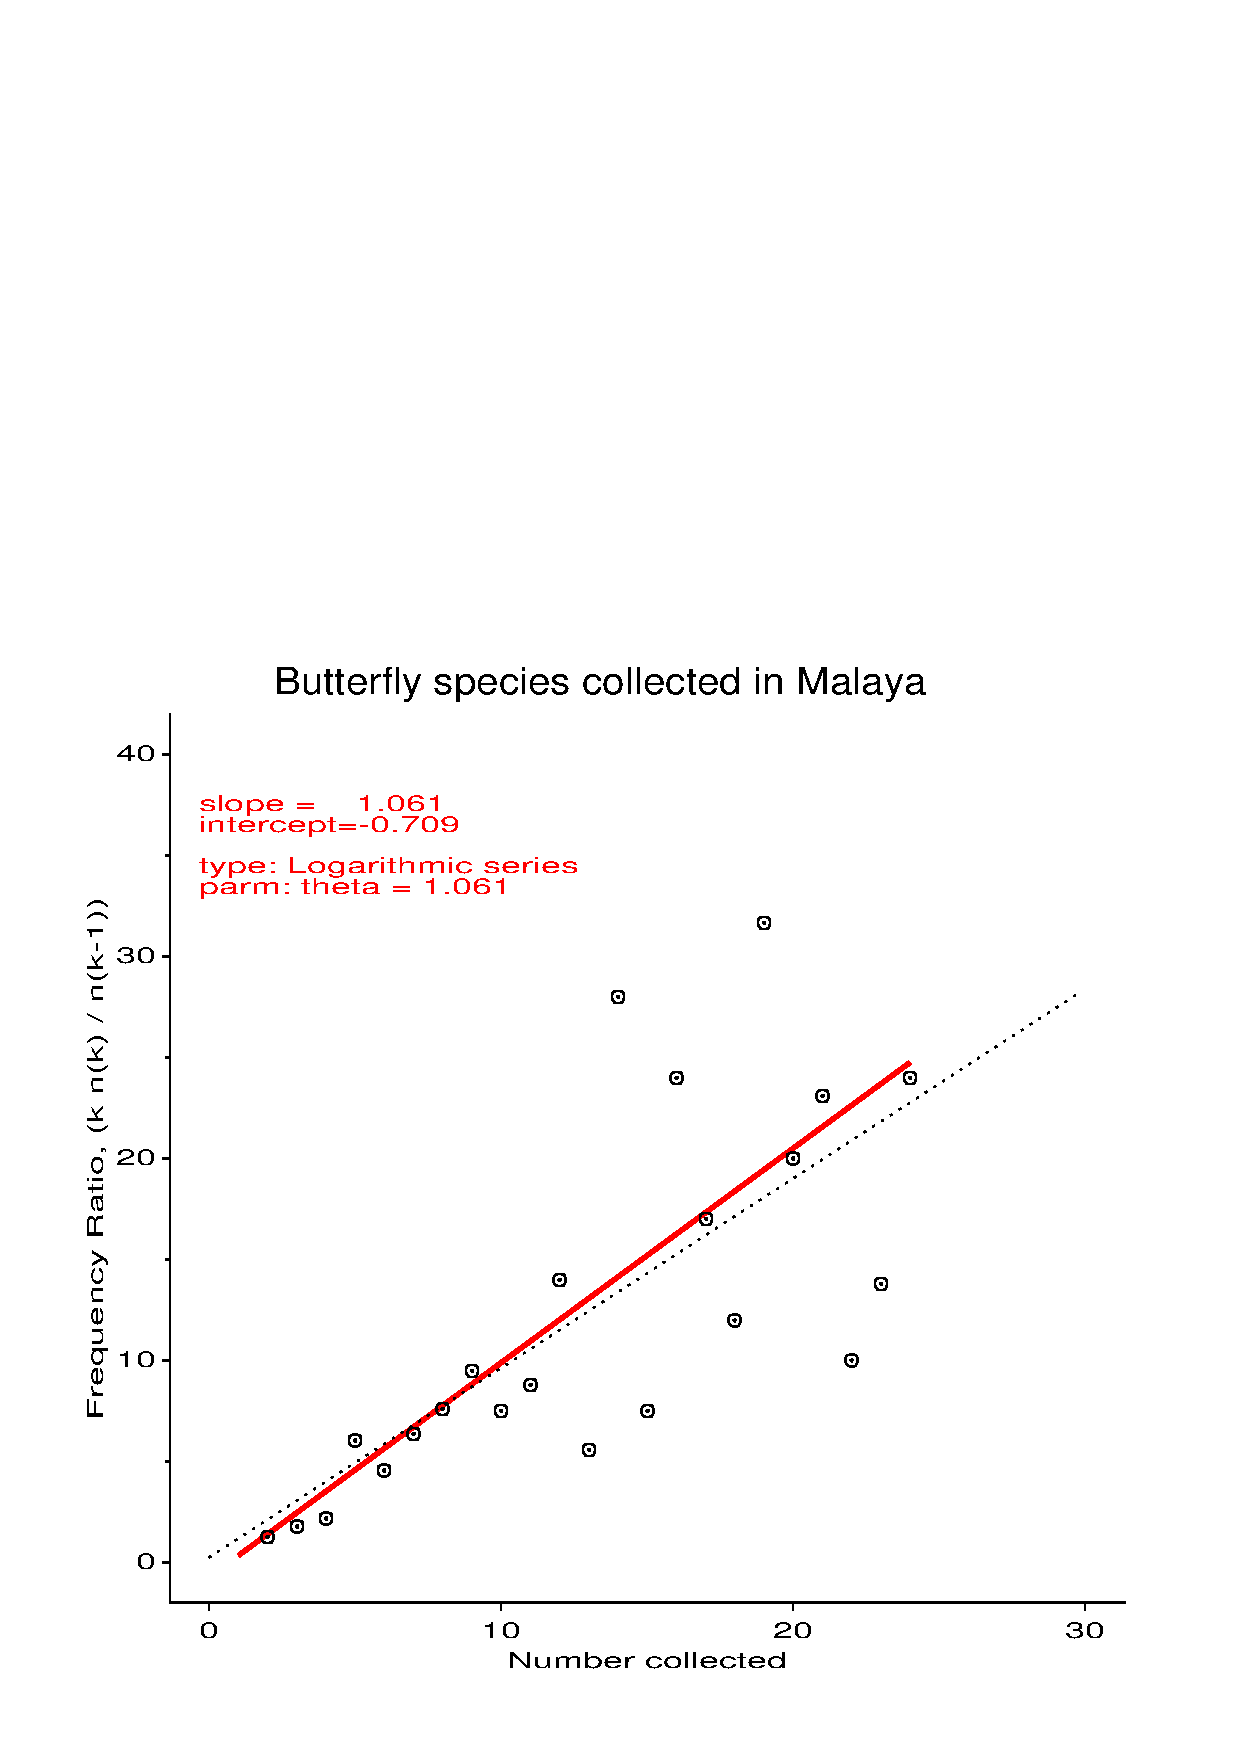
\includegraphics[trim=0 0 0 0,width=\linewidth,clip]{fig/orddemo3}
  \\ \centering Logarithmic series
 \end{minipage}%
 \hfill
 \begin{minipage}[c]{.49\dispwidth}
%  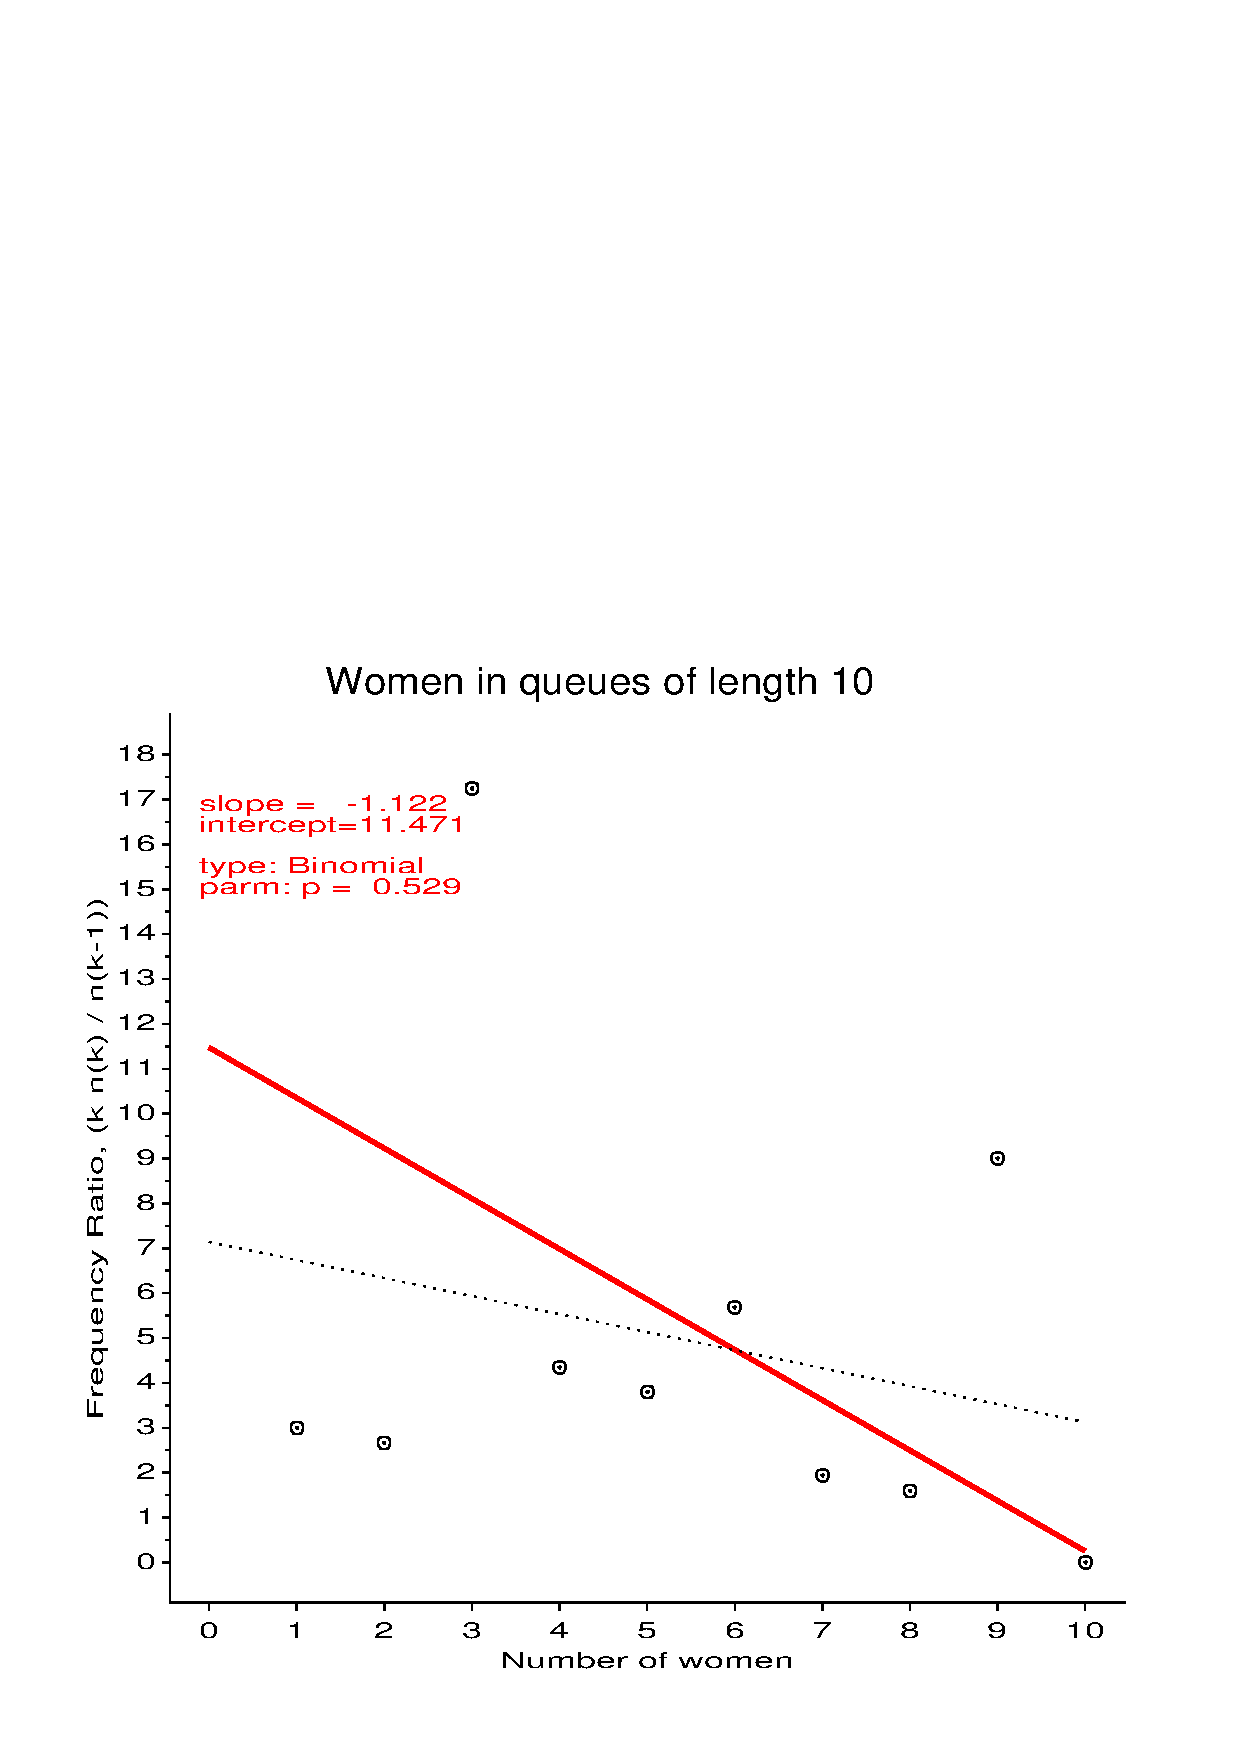
\includegraphics[trim=0 0 0 0,width=\linewidth,clip]{fig/orddemo4}
  \includegraphics[trim=0 0 0 0,width=\linewidth,clip]{fig/saxony4}
  \\ \centering Binomial
 \end{minipage}
\end{frame}

\subsection{Robust distribution plots}
\begin{frame}
  \frametitle{Robust distribution plots: Poisson}
  \begin{itemize}
	\item Ord plots lack robustness 
	\begin{itemize*}
	\item one discrepant freqency, $n_k$
	affects points for both $k$ and $k+1$
	\end{itemize*}

	\item Robust plots for Poisson distribution \citep{HoaglinTukey:85}
	\begin{itemize*}
	  \item For Poisson, plot \boldital{count metameter} =
	  \(\phi \,  ( n_k )  = \log_e ( k ! \,  n_k  /  N )\) vs.\ $k$
	  \item Linear relation $\Rightarrow$ Poisson, slope gives $\hat{\lambda}$
	  \item CI for points, diagnostic (influence) plot
	  \item \macro{POISPLOT}
	\end{itemize*}
  \end{itemize}
\end{frame}

\begin{frame}
  \frametitle{Poissonness plots: Details}
  \begin{itemize}
	\item If the distribution of $n_k$ is Poisson($\lambda$) for some fixed $\lambda$, then each
	observed frequency, $n_k \approx m_k = N p_k$.
	\item Then, setting
\(n_k = N p_k  = { e^{ - \lambda } \:  \lambda^k } /  { k ! }\),
and taking logs of both sides gives
  \[
  \log ( n_k ) = \log \,  N - \lambda  +  k \,  \log \,  \lambda  -
  \log \,  k !
  \]
which can be rearranged to
  \begin{equation*}
  \phi \,  ( n_k )  \equiv \log \left(  \frac{ k ! \:  n_k } {N} \right)
 = - \lambda  +  ( \log \,  \lambda ) \,  k
  \end{equation*}

	\item $\Rightarrow$ if the distribution is Poisson,
	plotting \(\phi ( n_k )\) vs.\ \(k\) should give a line with
	  \begin{itemize*}
	  \item intercept = \(- \lambda\)
	  \item slope = \(\log  \,  \lambda\)
	  \end{itemize*}
	\item Nonlinear relation $\rightarrow$ distribution is \emph{not} Poisson
    \item \citet{HoaglinTukey:85} give details on calculation of confidence intervals
	and influence measures.
  \end{itemize}
\end{frame}

\begin{frame}[fragile]
  \frametitle{\macrot{POISPLOT}: example}
  \begin{Input}[fontsize=\small]
title "Instances of 'may' in Federalist papers";
data madison;
   input count blocks;
   label count='Number of Occurrences'
         blocks='Blocks of Text';
datalines;
  0    156
  1     63
  2     29
  3      8
  4      4
  5      1
  6      1
;
\sasemph{%poisplot(data=madison,count=count, freq=blocks)};
  \end{Input}
\end{frame}

\begin{frame}
  \frametitle{\macrot{POISPLOT}: output}
Curvilinear relation $\rightarrow$ distribution is \emph{not} Poisson
 \begin{minipage}[c]{.49\dispwidth}
  \includegraphics[width=1\linewidth]{fig/poisdemo-mad}
  \\ \centering Poissonness plot
 \end{minipage}%
 \hfill
 \begin{minipage}[c]{.49\dispwidth}
  \includegraphics[width=1\linewidth]{fig/poisdemo-mad3}
  \\ \centering Influence plot for change in $\lambda$
 \end{minipage}

\end{frame}

\begin{frame}[fragile]
  \frametitle{Generalized robust distribution plots}
  Other distributions: Analogous plots, for suitable count metameter, 
  $\phi \,  ( n_k )$
  vs.\ $k$.
  \begin{itemize*}
  \item Linear relation $\Rightarrow$ correct distribution, slope gives parameter estimates
  \item CI reflect variability of the individual counts, $n_k$
  \item \macro{DISTPLOT}
  \end{itemize*}

  \begin{Code}
  %distplot(data=madison, count=count, freq=blocks,
        \sasemph{dist=negbin});
  \end{Code}

  \begin{center}
	\includegraphics[width=.5\dispwidth,clip]{fig/maddist}
  \end{center}
\end{frame}
